% Options for packages loaded elsewhere
\PassOptionsToPackage{unicode}{hyperref}
\PassOptionsToPackage{hyphens}{url}
%
\documentclass[
]{article}
\usepackage{amsmath,amssymb}
\usepackage{lmodern}
\usepackage{setspace}
\usepackage{iftex}
\ifPDFTeX
  \usepackage[T1]{fontenc}
  \usepackage[utf8]{inputenc}
  \usepackage{textcomp} % provide euro and other symbols
\else % if luatex or xetex
  \usepackage{unicode-math}
  \defaultfontfeatures{Scale=MatchLowercase}
  \defaultfontfeatures[\rmfamily]{Ligatures=TeX,Scale=1}
\fi
% Use upquote if available, for straight quotes in verbatim environments
\IfFileExists{upquote.sty}{\usepackage{upquote}}{}
\IfFileExists{microtype.sty}{% use microtype if available
  \usepackage[]{microtype}
  \UseMicrotypeSet[protrusion]{basicmath} % disable protrusion for tt fonts
}{}
\makeatletter
\@ifundefined{KOMAClassName}{% if non-KOMA class
  \IfFileExists{parskip.sty}{%
    \usepackage{parskip}
  }{% else
    \setlength{\parindent}{0pt}
    \setlength{\parskip}{6pt plus 2pt minus 1pt}}
}{% if KOMA class
  \KOMAoptions{parskip=half}}
\makeatother
\usepackage{xcolor}
\usepackage[margin=1in]{geometry}
\usepackage{color}
\usepackage{fancyvrb}
\newcommand{\VerbBar}{|}
\newcommand{\VERB}{\Verb[commandchars=\\\{\}]}
\DefineVerbatimEnvironment{Highlighting}{Verbatim}{commandchars=\\\{\}}
% Add ',fontsize=\small' for more characters per line
\usepackage{framed}
\definecolor{shadecolor}{RGB}{248,248,248}
\newenvironment{Shaded}{\begin{snugshade}}{\end{snugshade}}
\newcommand{\AlertTok}[1]{\textcolor[rgb]{0.94,0.16,0.16}{#1}}
\newcommand{\AnnotationTok}[1]{\textcolor[rgb]{0.56,0.35,0.01}{\textbf{\textit{#1}}}}
\newcommand{\AttributeTok}[1]{\textcolor[rgb]{0.77,0.63,0.00}{#1}}
\newcommand{\BaseNTok}[1]{\textcolor[rgb]{0.00,0.00,0.81}{#1}}
\newcommand{\BuiltInTok}[1]{#1}
\newcommand{\CharTok}[1]{\textcolor[rgb]{0.31,0.60,0.02}{#1}}
\newcommand{\CommentTok}[1]{\textcolor[rgb]{0.56,0.35,0.01}{\textit{#1}}}
\newcommand{\CommentVarTok}[1]{\textcolor[rgb]{0.56,0.35,0.01}{\textbf{\textit{#1}}}}
\newcommand{\ConstantTok}[1]{\textcolor[rgb]{0.00,0.00,0.00}{#1}}
\newcommand{\ControlFlowTok}[1]{\textcolor[rgb]{0.13,0.29,0.53}{\textbf{#1}}}
\newcommand{\DataTypeTok}[1]{\textcolor[rgb]{0.13,0.29,0.53}{#1}}
\newcommand{\DecValTok}[1]{\textcolor[rgb]{0.00,0.00,0.81}{#1}}
\newcommand{\DocumentationTok}[1]{\textcolor[rgb]{0.56,0.35,0.01}{\textbf{\textit{#1}}}}
\newcommand{\ErrorTok}[1]{\textcolor[rgb]{0.64,0.00,0.00}{\textbf{#1}}}
\newcommand{\ExtensionTok}[1]{#1}
\newcommand{\FloatTok}[1]{\textcolor[rgb]{0.00,0.00,0.81}{#1}}
\newcommand{\FunctionTok}[1]{\textcolor[rgb]{0.00,0.00,0.00}{#1}}
\newcommand{\ImportTok}[1]{#1}
\newcommand{\InformationTok}[1]{\textcolor[rgb]{0.56,0.35,0.01}{\textbf{\textit{#1}}}}
\newcommand{\KeywordTok}[1]{\textcolor[rgb]{0.13,0.29,0.53}{\textbf{#1}}}
\newcommand{\NormalTok}[1]{#1}
\newcommand{\OperatorTok}[1]{\textcolor[rgb]{0.81,0.36,0.00}{\textbf{#1}}}
\newcommand{\OtherTok}[1]{\textcolor[rgb]{0.56,0.35,0.01}{#1}}
\newcommand{\PreprocessorTok}[1]{\textcolor[rgb]{0.56,0.35,0.01}{\textit{#1}}}
\newcommand{\RegionMarkerTok}[1]{#1}
\newcommand{\SpecialCharTok}[1]{\textcolor[rgb]{0.00,0.00,0.00}{#1}}
\newcommand{\SpecialStringTok}[1]{\textcolor[rgb]{0.31,0.60,0.02}{#1}}
\newcommand{\StringTok}[1]{\textcolor[rgb]{0.31,0.60,0.02}{#1}}
\newcommand{\VariableTok}[1]{\textcolor[rgb]{0.00,0.00,0.00}{#1}}
\newcommand{\VerbatimStringTok}[1]{\textcolor[rgb]{0.31,0.60,0.02}{#1}}
\newcommand{\WarningTok}[1]{\textcolor[rgb]{0.56,0.35,0.01}{\textbf{\textit{#1}}}}
\usepackage{graphicx}
\makeatletter
\def\maxwidth{\ifdim\Gin@nat@width>\linewidth\linewidth\else\Gin@nat@width\fi}
\def\maxheight{\ifdim\Gin@nat@height>\textheight\textheight\else\Gin@nat@height\fi}
\makeatother
% Scale images if necessary, so that they will not overflow the page
% margins by default, and it is still possible to overwrite the defaults
% using explicit options in \includegraphics[width, height, ...]{}
\setkeys{Gin}{width=\maxwidth,height=\maxheight,keepaspectratio}
% Set default figure placement to htbp
\makeatletter
\def\fps@figure{htbp}
\makeatother
\setlength{\emergencystretch}{3em} % prevent overfull lines
\providecommand{\tightlist}{%
  \setlength{\itemsep}{0pt}\setlength{\parskip}{0pt}}
\setcounter{secnumdepth}{5}
\newlength{\cslhangindent}
\setlength{\cslhangindent}{1.5em}
\newlength{\csllabelwidth}
\setlength{\csllabelwidth}{3em}
\newlength{\cslentryspacingunit} % times entry-spacing
\setlength{\cslentryspacingunit}{\parskip}
\newenvironment{CSLReferences}[2] % #1 hanging-ident, #2 entry spacing
 {% don't indent paragraphs
  \setlength{\parindent}{0pt}
  % turn on hanging indent if param 1 is 1
  \ifodd #1
  \let\oldpar\par
  \def\par{\hangindent=\cslhangindent\oldpar}
  \fi
  % set entry spacing
  \setlength{\parskip}{#2\cslentryspacingunit}
 }%
 {}
\usepackage{calc}
\newcommand{\CSLBlock}[1]{#1\hfill\break}
\newcommand{\CSLLeftMargin}[1]{\parbox[t]{\csllabelwidth}{#1}}
\newcommand{\CSLRightInline}[1]{\parbox[t]{\linewidth - \csllabelwidth}{#1}\break}
\newcommand{\CSLIndent}[1]{\hspace{\cslhangindent}#1}
\ifLuaTeX
  \usepackage{selnolig}  % disable illegal ligatures
\fi
\IfFileExists{bookmark.sty}{\usepackage{bookmark}}{\usepackage{hyperref}}
\IfFileExists{xurl.sty}{\usepackage{xurl}}{} % add URL line breaks if available
\urlstyle{same} % disable monospaced font for URLs
\hypersetup{
  pdftitle={Pressure},
  pdfauthor={Sofia Russo},
  hidelinks,
  pdfcreator={LaTeX via pandoc}}

\title{Pressure}
\usepackage{etoolbox}
\makeatletter
\providecommand{\subtitle}[1]{% add subtitle to \maketitle
  \apptocmd{\@title}{\par {\large #1 \par}}{}{}
}
\makeatother
\subtitle{Relating temperature and pressure}
\author{Sofia Russo}
\date{Università degli Studi di Padova}

\begin{document}
\maketitle

{
\setcounter{tocdepth}{3}
\tableofcontents
}
\setstretch{1.5}
\hypertarget{dataset}{%
\section{DATASET}\label{dataset}}

\hypertarget{variable-pressure}{%
\subsection{Variable: pressure}\label{variable-pressure}}

\emph{Prova} \textbf{prova} \textbf{\emph{blablabla}}
\textcolor{red}{prova} \color{red}\Huge blablabla
\normalsize \normalcolor prova \Huge blablabla \normalsize  Epifania,
Anselmi, and Robusto (2021)

\begin{quote}
Prova prova blablabla Prova prova blablabla
\end{quote}

\begin{itemize}
\tightlist
\item
  Prova
\item
  prova

  \begin{enumerate}
  \def\labelenumi{\arabic{enumi}.}
  \tightlist
  \item
    Papappero

    \begin{enumerate}
    \def\labelenumii{\arabic{enumii}.}
    \tightlist
    \item
      Pappararra
    \end{enumerate}
  \end{enumerate}
\item
  blablabla
\end{itemize}

\begin{enumerate}
\def\labelenumi{\arabic{enumi}.}
\tightlist
\item
  Prova
\item
  prova
\item
  blablabla
\end{enumerate}

\hypertarget{inspection}{%
\subsubsection{Inspection}\label{inspection}}

Prova prova blablabla Prova prova blablabla Prova prova blablabla Prova
prova blablabla Prova prova blablabla Prova prova blablabla Prova prova
blablabla Prova prova blablabla Prova prova blablabla

\begin{itemize}
\tightlist
\item
  Prova

  \begin{itemize}
  \tightlist
  \item
    Mannaggia

    \begin{itemize}
    \tightlist
    \item
      Aaaaaa
    \end{itemize}
  \item
    Mannaggia
  \end{itemize}
\item
  Prova
\end{itemize}

Con i piedi\footnote{ciao ciao}

Con le mani \footnote{ciao}

\hypertarget{what-is-relevant-to-note-nothing}{%
\paragraph{What is relevant to note:
nothing}\label{what-is-relevant-to-note-nothing}}

prova \color{blue}\href{https://poterealpopolo.org/}{Link}\normalcolor

\hypertarget{oh-well-whatever-nevermind}{%
\paragraph{Oh well whatever:
nevermind}\label{oh-well-whatever-nevermind}}

\color{blue}\href{https://it.wikipedia.org/wiki/Cielo}{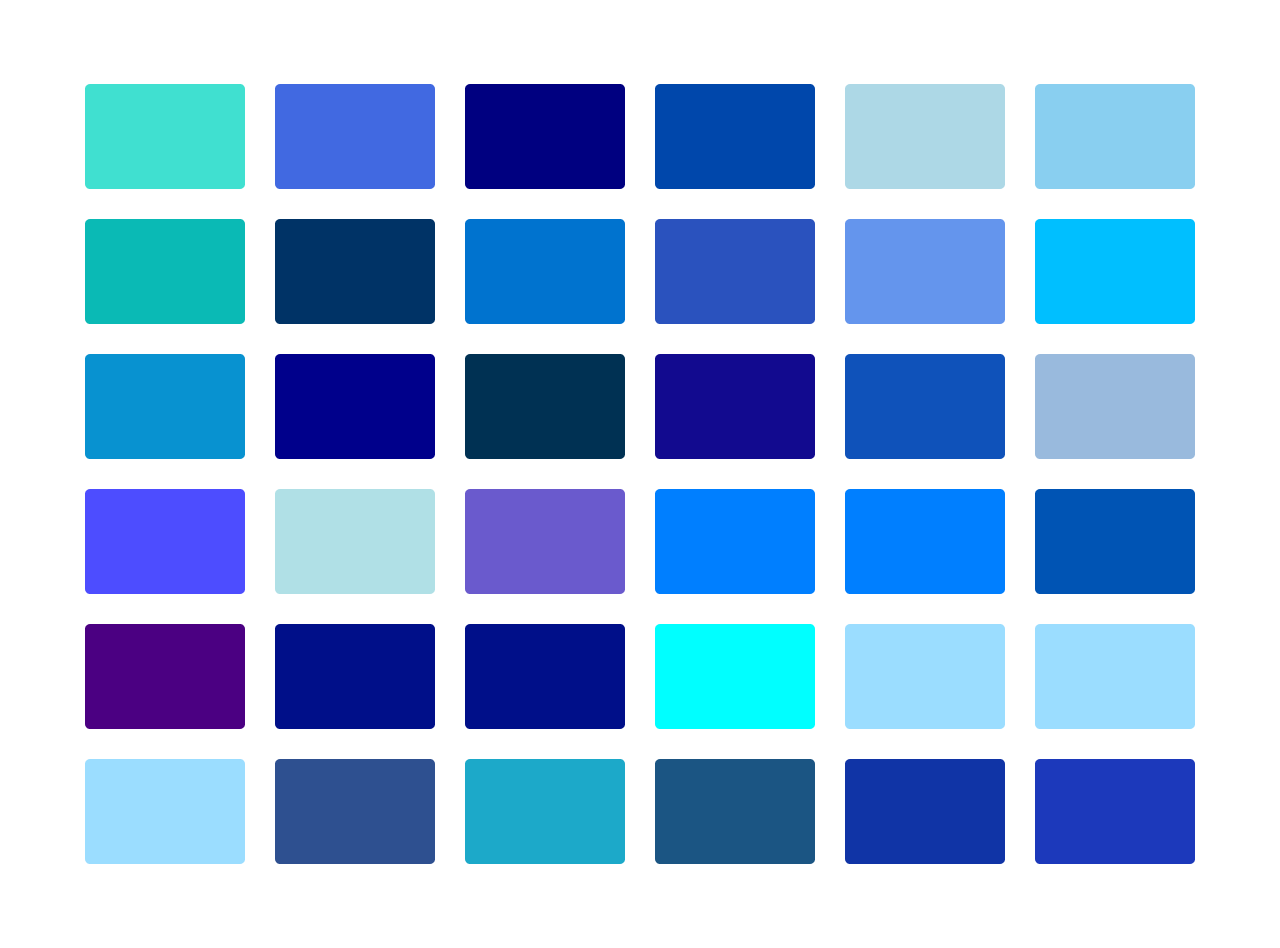
\includegraphics{images/blues.png}}\normalcolor
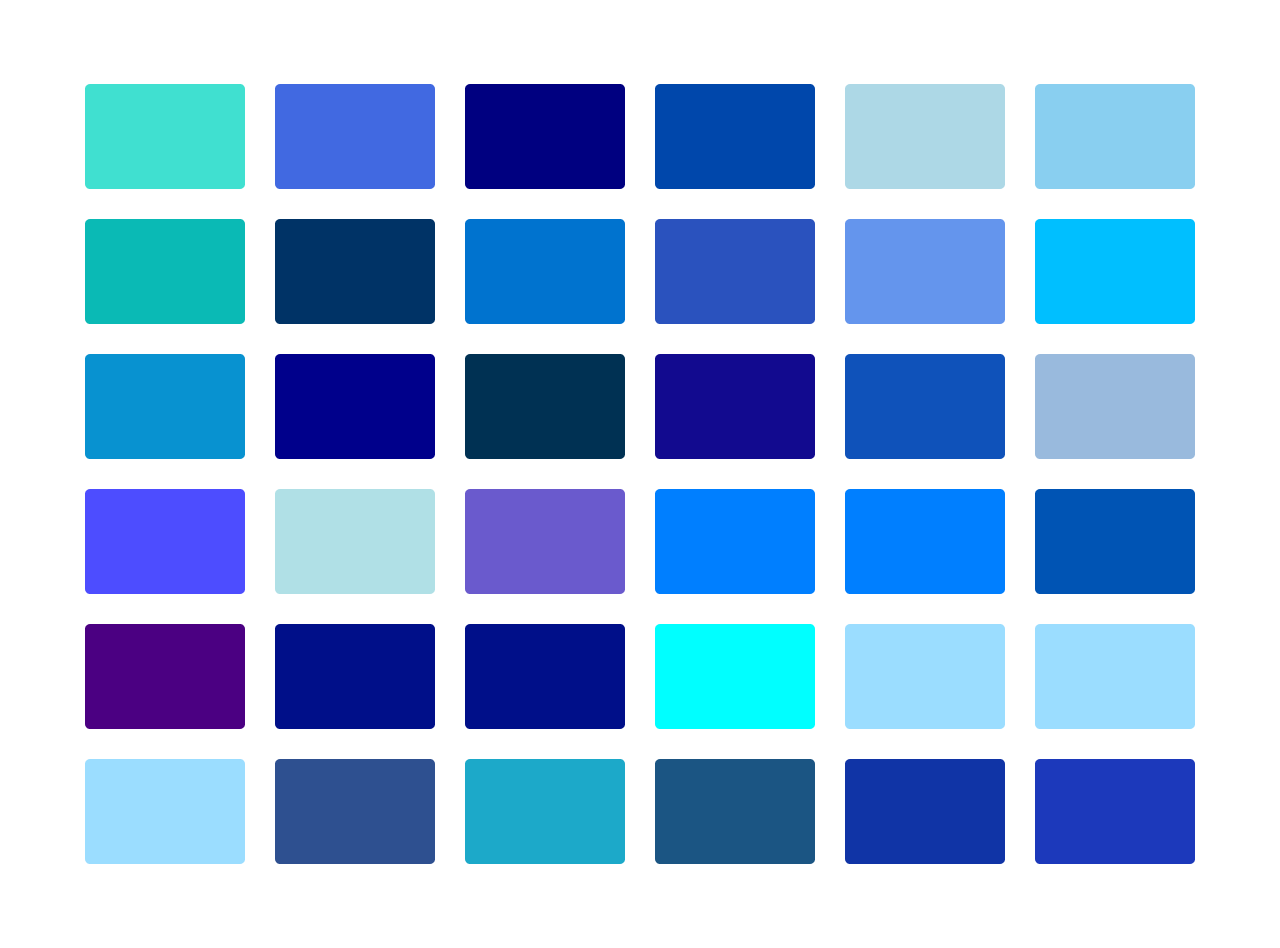
\includegraphics{images/blues.png}

\begin{Shaded}
\begin{Highlighting}[]
\NormalTok{knitr}\SpecialCharTok{::}\FunctionTok{include\_graphics}\NormalTok{(}\AttributeTok{path =} \StringTok{"images/earth\_core.jpeg"}\NormalTok{)}
\end{Highlighting}
\end{Shaded}

\begin{figure}

\hfill{}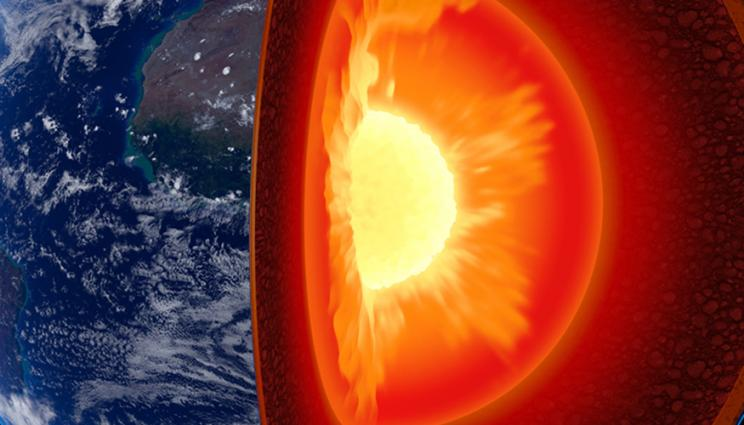
\includegraphics[width=0.1\linewidth]{images/earth_core} 

\caption{Caption}\label{fig:unnamed-chunk-1}
\end{figure}

\begin{verbatim}
lol   temperature pressure
lol 1           0   0.0002
lol 2          20   0.0012
lol 3          40   0.0060
lol 4          60   0.0300
lol 5          80   0.0900
lol 6         100   0.2700
\end{verbatim}

Questo è il dataset:

\begin{verbatim}
lol     Min.  1st Qu.   Median     Mean  3rd Qu.     Max. 
lol   0.0002   0.1800   8.8000 124.3367 126.5000 806.0000
\end{verbatim}

\begin{Shaded}
\begin{Highlighting}[]
\NormalTok{data}
\end{Highlighting}
\end{Shaded}

\begin{verbatim}
nonlol    temperature pressure   y        x
nonlol 1            0   0.0002   0   0.0002
nonlol 2           20   0.0012  20   0.0012
nonlol 3           40   0.0060  40   0.0060
....
\end{verbatim}

e questo è il plot grezzi:

\begin{center}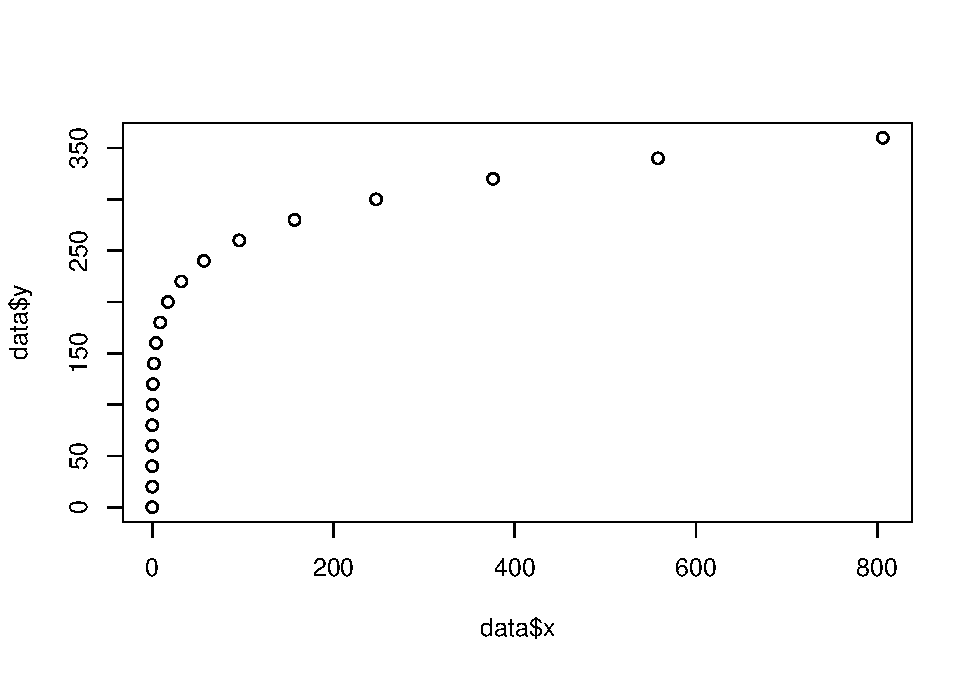
\includegraphics{Prova_knit_files/figure-latex/unnamed-chunk-5-1} \end{center}

mentre questo è la regressione applicata, con codice e risultati:

\begin{Shaded}
\begin{Highlighting}[]
\CommentTok{\# regressione}
\NormalTok{m }\OtherTok{=} \FunctionTok{lm}\NormalTok{(y }\SpecialCharTok{\textasciitilde{}}\NormalTok{ x, }\AttributeTok{data =}\NormalTok{ data)}
\CommentTok{\# summary del modello}
\FunctionTok{summary}\NormalTok{(m)}
\end{Highlighting}
\end{Shaded}

\begin{verbatim}
lol 
lol Call:
lol lm(formula = y ~ x, data = data)
lol 
lol Residuals:
lol      Min       1Q   Median       3Q      Max 
lol -132.791  -62.813    6.507   67.033   90.759 
lol 
lol Coefficients:
lol              Estimate Std. Error t value Pr(>|t|)    
lol (Intercept) 132.79072   19.94314   6.658 4.03e-06 ***
lol x             0.37969    0.07929   4.788 0.000171 ***
lol ---
lol Signif. codes:  0 '***' 0.001 '**' 0.01 '*' 0.05 '.' 0.1 ' ' 1
lol 
lol Residual standard error: 75.56 on 17 degrees of freedom
lol Multiple R-squared:  0.5742,    Adjusted R-squared:  0.5492 
lol F-statistic: 22.93 on 1 and 17 DF,  p-value: 0.000171
\end{verbatim}

\begin{table}[!htbp] \centering 
  \caption{Tabella di summary} 
  \label{} 
\begin{tabular}{@{\extracolsep{5pt}}lccccc} 
\\[-1.8ex]\hline 
\hline \\[-1.8ex] 
Statistic & \multicolumn{1}{c}{N} & \multicolumn{1}{c}{Mean} & \multicolumn{1}{c}{St. Dev.} & \multicolumn{1}{c}{Min} & \multicolumn{1}{c}{Max} \\ 
\hline \\[-1.8ex] 
temperature & 19 & 180.00 & 112.55 & 0 & 360 \\ 
pressure & 19 & 124.34 & 224.62 & 0.0002 & 806.00 \\ 
y & 19 & 180.00 & 112.55 & 0 & 360 \\ 
x & 19 & 124.34 & 224.62 & 0.0002 & 806.00 \\ 
\hline \\[-1.8ex] 
\end{tabular} 
\end{table}

\begin{table}[!htbp] \centering 
  \caption{Risultati del modello} 
  \label{} 
\begin{tabular}{@{\extracolsep{5pt}}lc} 
\\[-1.8ex]\hline 
\hline \\[-1.8ex] 
 & \multicolumn{1}{c}{\textit{Dependent variable:}} \\ 
\cline{2-2} 
\\[-1.8ex] & y \\ 
\hline \\[-1.8ex] 
 x & 0.38$^{***}$ \\ 
  & (0.08) \\ 
  & \\ 
 Constant & 132.79$^{***}$ \\ 
  & (19.94) \\ 
  & \\ 
\hline \\[-1.8ex] 
Observations & 19 \\ 
R$^{2}$ & 0.57 \\ 
Adjusted R$^{2}$ & 0.55 \\ 
Residual Std. Error & 75.56 (df = 17) \\ 
F Statistic & 22.93$^{***}$ (df = 1; 17) \\ 
\hline 
\hline \\[-1.8ex] 
\textit{Note:}  & \multicolumn{1}{r}{$^{*}$p$<$0.1; $^{**}$p$<$0.05; $^{***}$p$<$0.01} \\ 
\end{tabular} 
\end{table}

\begin{table}[!htbp] \centering 
\begin{tabular}{@{\extracolsep{5pt}}lcc} 
\\[-1.8ex]\hline 
\hline \\[-1.8ex] 
 & \multicolumn{2}{c}{\textit{Dependent variable:}} \\ 
\cline{2-3} 
\\[-1.8ex] & \multicolumn{2}{c}{temperature} \\ 
\\[-1.8ex] & (1) & (2)\\ 
\hline \\[-1.8ex] 
 Constant & 180.00$^{***}$ & 132.79$^{***}$ \\ 
  & (25.82) & (19.94) \\ 
  & & \\ 
 pressure &  & 0.38$^{***}$ \\ 
  &  & (0.08) \\ 
  & & \\ 
\hline \\[-1.8ex] 
Observations & 19 & 19 \\ 
R$^{2}$ & 0.00 & 0.57 \\ 
Adjusted R$^{2}$ & 0.00 & 0.55 \\ 
Residual Std. Error & 112.55 (df = 18) & 75.56 (df = 17) \\ 
F Statistic &  & 22.93$^{***}$ (df = 1; 17) \\ 
\hline 
\hline \\[-1.8ex] 
\textit{Note:}  & \multicolumn{2}{r}{$^{*}$p$<$0.1; $^{**}$p$<$0.05; $^{***}$p$<$0.01} \\ 
\end{tabular} 
  \caption{Model comparison} 
  \label{} 
\end{table}

Formule

\(z = \frac{x_i - \bar{X}}{sd} = \frac{\ensuremath{2\times 10^{-4}}- 124.3367053}{224.6225399 } = -0.5533362\)

\begin{Shaded}
\begin{Highlighting}[]
\NormalTok{x }\OtherTok{=}\NormalTok{ data}\SpecialCharTok{$}\NormalTok{pressure}
\NormalTok{y }\OtherTok{=}\NormalTok{ data}\SpecialCharTok{$}\NormalTok{temperature}
\end{Highlighting}
\end{Shaded}

\$ y = \left(\frac{a}{b})\right \^{}2\$

\hypertarget{refs}{}
\begin{CSLReferences}{1}{0}
\leavevmode\vadjust pre{\hypertarget{ref-epifania2021implicit}{}}%
Epifania, Ottavia M, Pasquale Anselmi, and Egidio Robusto. 2021.
{``Implicit Social Cognition Through the Years: The Implicit Association
Test at Age 21.''} \emph{Psychology of Consciousness: Theory, Research,
and Practice}.

\end{CSLReferences}

\end{document}
